\documentclass{beamer} 
\usetheme{Madrid} % My favorite! 
%\usetheme{Boadilla} 
% Pretty neat, soft color. 
%\usetheme{default} 
%\usetheme{Warsaw} 
%\usetheme{Bergen} 
% This template has nagivation on the left 
%\usetheme{Frankfurt} % Similar to the default 
% with an extra region at the top. 
%\usecolortheme{seahorse} % Simple and clean template 
%\usetheme{Darmstadt} % not so good 
% Uncomment the following line if you want 
% % page numbers and using Warsaw theme%
% \setbeamertemplate{footline}[page number] 
%\setbeamercovered{transparent} 
\setbeamercovered{invisible} % To remove the navigation symbols from 
% the bottom of slides
% \setbeamertemplate{navigation symbols}{} 
\usepackage{graphicx} 
%\usepackage{bm} % For typesetting bold math (not \mathbold) 
%\logo{\includegraphics[height=0.6cm]{yourlogo.eps}} % 
\title[Quantised Calculus]{Quantised Calculus in One Variable} 
\author{E McDonald} 
\institute[UNSW] { UNSW Australia } 
\titlegraphic{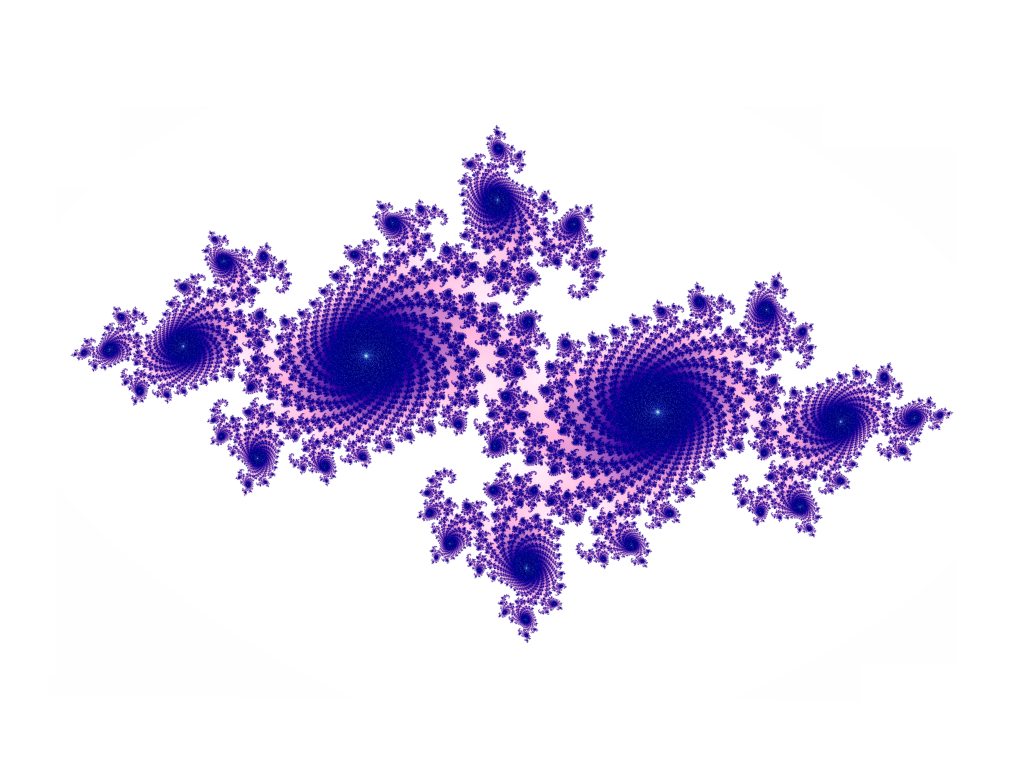
\includegraphics[width=60mm]{Julia_set_(ice).png}}

\date{\today} 



% \today will show current date. 
% Alternatively, you can specify a date. 


\begin{document} 


\begin{frame} 
\titlepage 
\end{frame} % 



\begin{frame} 

\frametitle{Motivation} 

\begin{block} 
{Question: What is Quantised Calculus?} 
Answer: A generalisation of ordinary calculus
\end{block}

\end{frame} % 

\begin{frame} 
\frametitle{Example of a Theorem} 
\begin{theorem}
The quick brown fox jumps over the lazy dog. 
\end{theorem}
\end{frame} 

\begin{frame} 

\centerline{The End} 

\end{frame} % End of slides \end{document} - See more at: http://www.stattler.com/article/ready-made-beamer-presentation-template#sthash.lLGVQYLI.dpuf

\end{document}